\section{Design considerations}
\label{section:design}

%\subsection{Multipath state}
%\subsection{Network granularity}
%\subsection{Deployment}
%\subsection{Flowlet?}

\ac{SDN} provides an abstraction over which different architectural paradigms can be adapted and even coexist.
It does not however prescribe or advocate a specific design -- network practitioners must still consider system properties when grappling with fundamental tradeoffs affecting consistency, isolation, reliability and efficiency.
This section provides design considerations for scalable traffic management based on observations obtained from the data collected in chapters \ref{chapter:malawi} and \ref{chapter:rate}.

\begin{figure}[t]
    \centering
    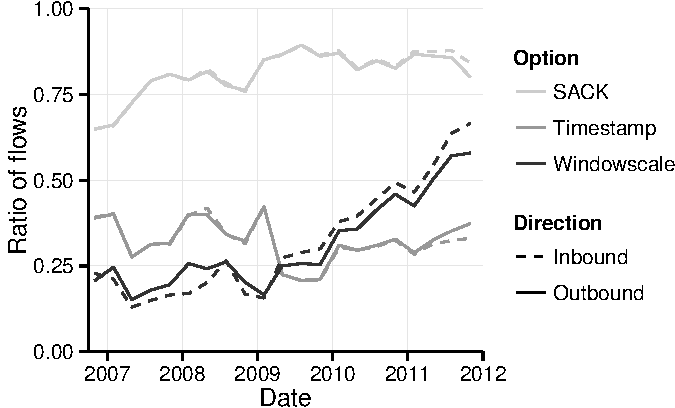
\includegraphics[width=4.0in]{figures/inflex/options}
    \caption{\acs{TCP} option usage \label{fig:wscale}}
    \hfill
\end{figure}

Ideally resilience could be implemented at the transport layer alone, for the same motives rate control is best left to end-hosts: ultimately, the host is best positioned to detect end-to-end path faults and can often react over shorter timescales than the network, which must concern itself with reconvergence.
This approach for path fail-over was a significant feature in \ac{SCTP} \cite{rfc4960}.
Unfortunately, deployment of \ac{SCTP} has been negligible in over a decade since standardization, in part because the pervasiveness of middleboxes has significantly affected the ability for new transport protocols to be deployed.
More recently \ac{MPTCP} \cite{Wischik:2008p137} has been proposed addressing many of the same concerns as \ac{SCTP} whilst maintaining the same wire format as \ac{TCP}, thereby ensuring middlebox compatibility.
Despite this, widespread deployment is far from guaranteed, and is largely tied to the rate of \ac{OS} adoption.
As a reference point, figure \ref{fig:wscale} tracks the use of three \ac{TCP} options by overall volume in flows across both directions in the \ac{MAWI} dataset.
While \ac{SACK} is successfully negotiated for most connections, the deployment of the timestamp and windowscale options has lagged.
While the former primarily assists in provide more accurate \ac{RTT} estimates, the latter is critical for performance: without windowscale negotiation, a sender's congestion window cannot exceed 65KB.
Despite offering a clear benefit to both endpoints, being simple to implement and incurring a low overhead, windowscale deployment has only recently picked up momentum, two decades since standardization.
Expecting substantial deployment of a more complex and costly extension such as \ac{MPTCP} over the near future is likely optimistic.
Critically, transport extensions require receiver adoption and are therefore subject to the willingness and ability of users to upgrade their OS.

{\COMMENT missing: PREFLEX problems here. Concept of deployability changed.}

\textbf{Receiver side deployment of even modest \ac{TCP} extensions can be protracted, even when incentives are aligned}. 
Rather than proposing a path for incremental deployment, this work focuses on how to obtain similar benefits immediately -- modifying sender side hosts only. 
A host, however, cannot directly affect routing without changing destination address, which would break legacy \ac{TCP} receiver side implementations. Additional extensions are required on the sender side network to enable multipath forwarding.
Conventional wisdom suggests that maintaining parallel routing planes requires a proportional increase in table size \cite{NingWang:2008p145}, which itself can be subject to exponential growth.
In practice however, this state can be significantly reduced by forsaking coverage for a small proportion of traffic.
Rather than reflect the entirety of its potential path diversity for all traffic, an edge provider can instead provide additional routing planes for only a subset of popular prefixes.

\begin{figure}[t]
    \begin{subfigure}[b]{0.5\linewidth}
        \centering
        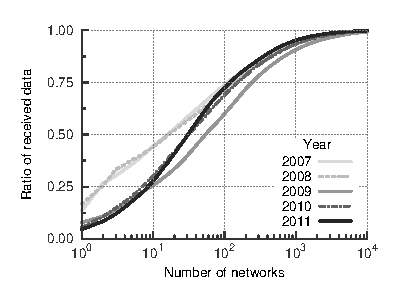
\includegraphics[width=3.0in]{figures/inflex/ecdf_network_dst_data_bytes_from_10000.eps}
        \caption{\label{prefix_in}}
    \end{subfigure}
    \begin{subfigure}[b]{0.5\linewidth}
        \centering
        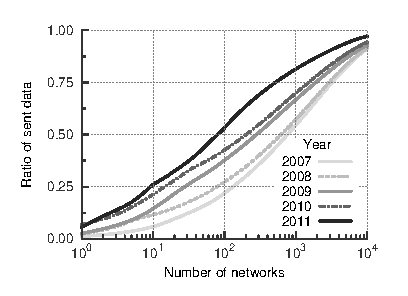
\includegraphics[width=3.0in]{figures/inflex/ecdf_network_dst_data_bytes_to_10000.eps}
        \caption{\label{prefix_out}}
    \end{subfigure}%
    \caption{\acs{CDF} of traffic by announced network prefix for (\subref{prefix_in}) inbound and (\subref{prefix_out}) outbound traffic.\label{fig:prefix}}
    \hfill
\end{figure}

The extent to which such a gain is possible for the \ac{MAWI} dataset is quantified in figure \ref{fig:prefix}, which displays the cumulative distribution function of outbound traffic across network prefixes announced by BGP neighbours.
Over five years, traffic to approximately 340,000 unique prefixes was observed.
Invariably however, an increasing amount is sent to a small group of prefixes -- by 2011, over 50\% of traffic went to the top 100 prefixes alone.
This reflects ongoing structural changes in the Internet architecture as content providers interconnect directly edge, \emph{eyeball} networks, and content becomes increasingly consolidated across a set of large content providers and national and regional ISPs.

\textbf{Multipath routing state can be significantly reduced by covering fewer destinations while still benefiting most traffic}. 
Within the \ac{MAWI} dataset virtually all inbound and outbound traffic could be mapped to 10,000 unique network prefixes. 
Existing \ac{SDN} tools such as RouteFlow \cite{Rothenberg:2012:RRC:2342441.2342445} are already capable of overlaying routing on commodity switches, but the incurred overhead can still be a concern for production networks.
Rather than address the scalability challenges inherent to multipath routing directly, these results suggest that a tangible deployment path lies instead in reducing the scope over which it is applied.

